\documentclass[utf8,xcolor=table]{beamer}

\usepackage[T2A]{fontenc}
\usepackage[utf8]{inputenc}
\usepackage[english,russian]{babel}
\usepackage{minted}
\usepackage{ulem}
\usepackage{cmap}
\usepackage{multirow}

\hypersetup{colorlinks,linkcolor=blue,urlcolor=blue}

\mode<presentation>{
	\usetheme{CambridgeUS}
}

\renewcommand{\t}[1]{\ifmmode{\mathtt{#1}}\else{\texttt{#1}}\fi}

\title{Арифметика в компьютерах}
\author{Егор Суворов}
\institute[СПб АУ]{Курс <<Парадигмы и языки программирования>>, подгруппа 3}
\date[17.10.2016]{Понедельник, 16 октября 2016 года}

\setlength{\arrayrulewidth}{1pt}

\begin{document}

\begin{frame}
\titlepage
\end{frame}

\begin{frame}{План занятия}
	\tableofcontents
\end{frame}

\section{Целые числа}
\subsection{Физическая часть}

\begin{frame}
	\tableofcontents[currentsection,currentsubsection]
\end{frame}

\begin{frame}
	Упрощённое представление о происходящем в <<железе>>:
	\begin{enumerate}
		\item Любой сигнал (в том числе бит) "--- это напряжение на проводе.
		\item Два уровня напряжения распознавать проще, чем три.
		\item Но три \href{https://ru.wikipedia.org/wiki/\%D0\%A1\%D0\%B5\%D1\%82\%D1\%83\%D0\%BD\%D1\%8C\_(\%D0\%BA\%D0\%BE\%D0\%BC\%D0\%BF\%D1\%8C\%D1\%8E\%D1\%82\%D0\%B5\%D1\%80)}{тоже было}, не прижилось.
		\item Вся логика построена на основе бинарных функций <<И>>, <<ИЛИ>> и остальных (\textit{гейты})
		\item Чем меньше гейтов "--- тем быстрее работает, тем меньше схема.
		\item Числа надо складывать, вычитать, умножать, делить, сравнивать на равенство и меньше/больше.
	\end{enumerate}
\end{frame}

\subsection{Типы данных}
\begin{frame}{Играем в игру}
	Чему соответствует бинарная запись в таблице ниже?

	Используйте калькулятор или Python: \t{0b0100} и \t{int('1111', 2)}.
	\begin{center}
		\pause
		\begin{tabular}{|c|c|}
			\hline
			\t{0001 0110} & \pause 22 \\\hline\noalign{\pause}
			\t{1000 0010} & \pause 130 \\\hline\noalign{\pause}
			\t{1000 0010} & \pause -126 \\\hline\noalign{\pause}
			\t{0011 0000} & \pause 48 \\\hline\noalign{\pause}
			\t{0011 0000} & \pause '0' \\\hline\noalign{\pause}
			\t{1100 0011} & \pause \t{0xC3} \\\hline\noalign{\pause}
			\t{1100 0011} & \pause \t{ret} \\\hline\noalign{\pause}
			\t{0110 1000} & \pause 22 \\
			\hline
		\end{tabular}
		\pause
	\end{center}
	Мораль: битовое представление ничего не говорит, если мы не договорились о том,
	как его интерпретировать (<<тип>>).

	Более того, представлений у одной и той же сущности может быть в
	некотором смысле много (\t{0xC3}, 195, \t{ret}).
\end{frame}

\begin{frame}{Ликбез-1}
	\begin{itemize}
		\item Основные типы чисел: целое, с фиксированной запятой, с плавающей запятой.
		\item Про строки и кодировки не говорим, там тоже довольно весело и интересно.
		\item Железо сейчас в основном поддерживает целые числа и с плавающей запятой.
		\item Железо умеет получать доступ к байту в памяти по его \textit{адресу}.
		\item Считаем, что адрес "--- это некоторое целое неотрицательное число.
	\end{itemize}
\end{frame}

\begin{frame}{Ликбез-2}
	\begin{itemize}
		\item
			Железо не может адресовать что-то внутри байта (биты).
		\item
			Но мы можем выполнять какие-то арифметические операции с байтами.
		\item
			Про порядок бит внутри байта говорить бессмысленно "--- мы никак его не проверим, у нас есть только арифметические операции.
		\item
			Будем рисовать \textit{младшие}/\textit{менее значимые} биты справа, как будто нормальные числа):
			\[ \t{0001 0010}_2 = 18_{10} \]
		\item
			Если какая-то конструкция занимает несколько байт подряд, то важно, в каком порядке они идут.
		\item
			Будем рисовать память слева направа: нулевой байт, первый...
	\end{itemize}
\end{frame}

\subsection{Беззнаковые числа}

\begin{frame}
	\tableofcontents[currentsection,currentsubsection]
\end{frame}

\begin{frame}[t]{Один байт}
	\begin{itemize}
		\item
			Любое целое число можно представить в двоичной системе счисления:
			\[ 150 = 128 + 16 + 4 + 2 = \t{1001~0110}_2 \]
		\item
			Есть младшие (менее значимые) знаки/биты, есть старшие.
		\item
			На ближайших слайдах работаем внутри 1 байта (8 бит).
		\item
			Пока все промежуточные результаты вычислений от $0$ до $255$, нет никаких проблем "--- считаем и считаем.
	\end{itemize}
	Что делать, если произошло переполнение (overflow/underflow)?
	Результат точно не сохраним.
	\begin{enumerate}
		\item Можно вызвать ошибку.
		\item Можно откинуть младшие знаки.
		\item Можно откинуть старшие знаки.
	\end{enumerate}
	Если откинем младшие, то $255+1-1\neq 255$, что неудобно, если мы хотим точные вычисления.
\end{frame}

\begin{frame}
	\begin{center}
		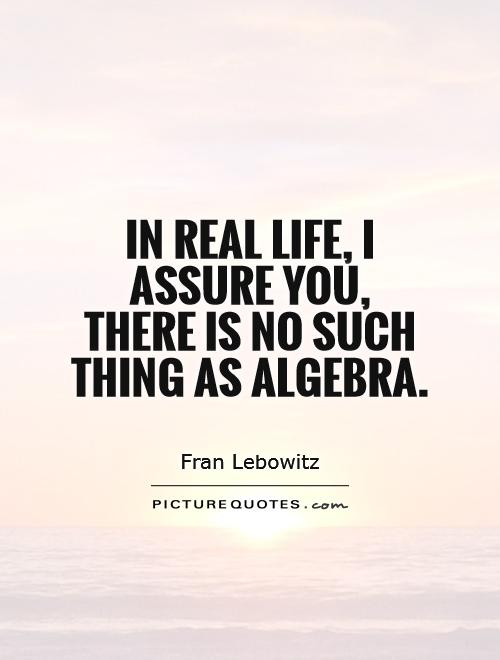
\includegraphics[scale=0.3]{will-i-use-algebra.jpg}
	\end{center}
\end{frame}

\begin{frame}
	А вот если считаем, что откидываем старшие, то получаем коммутативное кольцо с единицей $\mathbb{Z}/256\mathbb{Z}$.

	\begin{center}
		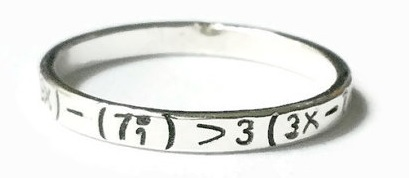
\includegraphics[scale=0.5]{math-ring.jpg}
	\end{center}

	\begin{itemize}
		\item
			По сути "--- просто арифметика, где все числа берутся по модулю 256.
		\item
			Сложение, вычитание, умножение в таких объектах прекрасно определены и непротиворечивы.
		\item
			Можно делать что угодно, и мы всегда получим корректный результат по модулю 256.
		\item
			В железе реализовать просто "--- считаем только последние 8 бит результата.
	\end{itemize}
\end{frame}

\begin{frame}{Деление}
	С делением хуже (деление "--- обратное к умножению).

	После взятия по модулю иногда можно однозначно восстановить ответ, а иногда нет (на алгебре расскажут, когда):
	\begin{align*}
	    34 / 17 &= 2 \\
		4386 / 17 &= 258 = 2 \mod 256 \\
		48 / 4 &= 12 \\
		\underbrace{(256+48)}_{304} / 4 &= 76
	\end{align*}
	Поэтому деление всегда считает, что у нас числа помещаются в 8 бит, и делим мы с остатком.
\end{frame}

\subsection{Знаковые числа}

\begin{frame}
	\tableofcontents[currentsection,currentsubsection]
\end{frame}

\begin{frame}
	\begin{itemize}
		\item
			Можно сказать, что в первом бите храним знак, а в остальных "--- число, как раньше (\textit{прямой код}).
		\item
			Тогда надо разбирать случаи в процессоре для всех арифметических и логических операций.
		\item
			Появляются $+0$ и $-0$, так что ещё и сравнение на равенство сильно менять.
	\end{itemize}

	А можно сказать, что, $-x$ по определению "--- это такое $y$, что $x+y=0$.

	Тогда вспоминаем, что мы уже живём по модулю 256 (проверьте вычисления в Python самостоятельно!):
	\begin{align*}
		x &= x + 256 &\mod 256 \\
		-56 &= -56 + 256 = 200 &\mod 256 \\
		-56 + 56 &= -56 + 256 + 56 = 256 = 0 &\mod 256 \\
		-17 \cdot 22 &= -374 = 138 &\mod 256 \\
		-17 \cdot 22 &= (256 - 17) \cdot 22 = 239 \cdot 22 = 5258 = 138 &\mod 256
	\end{align*}
\end{frame}

\begin{frame}
	\begin{center}
		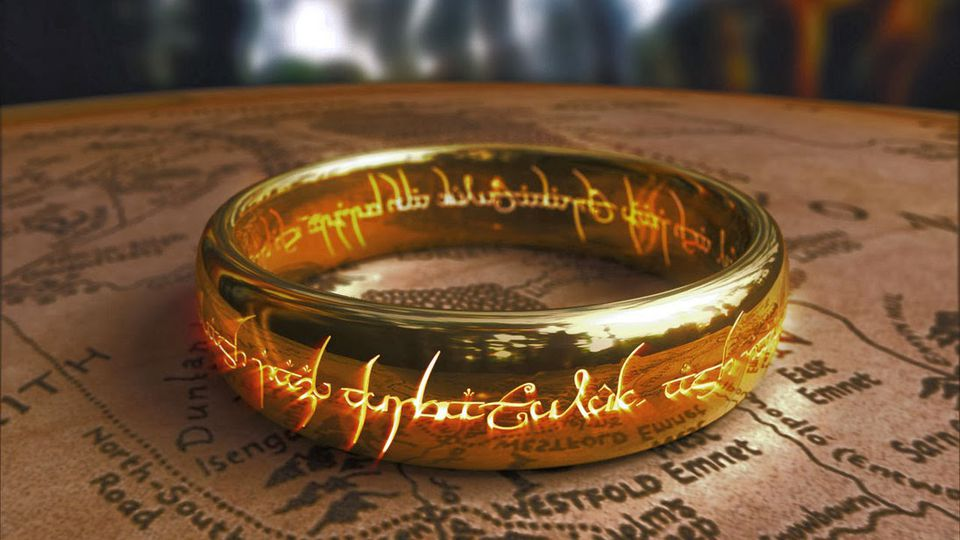
\includegraphics[scale=0.3]{one-ring-to-rule.jpg}
	\end{center}
\end{frame}

\begin{frame}
	Алгебра говорит, что $-x$ "--- это \textit{обратный по сложению к $x$}.
	В кольцах он есть.
	Считаем, что обратный по сложению к $x$ в кольце $\mathbb{Z}/256\mathbb{Z}$ и есть элемент $-x$.

	Мы только поменяли, как мы интерпретируем числа, но не их битовую запись:
	\begin{gather*}
		\mod 256 \\
		-56 + 100 = -56 + 256 + 100 = 200 + 100 = \\
		= \t{1100~1000} + \t{0110~0100} = \t{1~0010~1100} = \t{0010~1100} = 44
	\end{gather*}
	Таким образом, сложение, вычитание, и даже умножение по-прежнему работают (спасибо алгебраистам, что доказали).

	Упражнение: проверить, что:
	\[ a = b \mod 256 \rightarrow a \cdot x = b \cdot x \mod 256\]

	С делением хуже:
	\[
		-10 / 5 = (256 - 10) / 5 = 246 / 5 = 49.5 = \t{???}
	\]
\end{frame}

\begin{frame}{Дополнительный код}
	\begin{enumerate}
		\item Мы можем как угодно обозначить элементы кольца: какие-то назвать отрицательными числами, а какие-то "--- положительными.
		\item Обычно разделяют отрезок ровно пополам: $[-128; 127]$.
		\item Теперь по самому старшему биту можно определить знак: 1 "--- отрицательное, 0 "--- неотрицательное.
	\end{enumerate}

	Такая конвенция называется \textit{дополнительный код}: отрицательное и положительно число в сумме дают нули или
	дополняют до степени двойки $2^8$.

	\begin{enumerate}
		\item
			Надо разбирать случаи в сравнении чисел и в делении с остатком (поэтому они в ассемблере появляются знаковые/беззнаковые).
		\item
			Есть операция смены знака: инвертировать все биты и добавить единицу (инвертация бит "--- это вычитание из $\t{1111~1111}_2=255_{10}$).
	\end{enumerate}
\end{frame}

\begin{frame}{Упражнение}
	Как представлены следующие числа в дополнительном коде?

	\begin{center}
		\pause
		\begin{tabular}{|c|c|}
			\hline
			-1 & \pause \t{1111 1111} \\\hline\noalign{\pause}
			-128 & \pause \t{1000 0000} \\\hline\noalign{\pause}
			127 & \pause \t{0111 1111} \\\hline\noalign{\pause}
			128 & \pause никак \\
			\hline
		\end{tabular}
		\pause
	\end{center}
	Что будет, если мы возьмём $-(-128)$? \pause
	\begin{gather*}
		-128=\t{1000~0000} \\
		-(-128)=(\tilde{}\t{1000~0000})+1 = \t{0111~1111}+1 = \t{1000~0000} = 128 \\
	\end{gather*}
\end{frame}

\subsection{Порядок байт}

\begin{frame}
	\tableofcontents[currentsection,currentsubsection]
\end{frame}

\begin{frame}{Играем в игру}
	Напоминание: порядок бит в байте мы из программы никак не определим, на картинке рисуем слева старшие, справа младшие.

	Порядок байт в памяти "--- слева меньшие адреса, справа большие.

	\begin{center}
		\pause
		\begin{tabular}{|c|c|c|c|l|}
			\hline
			\multicolumn{4}{|c|}{Адрес} & Значение \\
			 & 2 & 3 & & \\\hline
			\dots & \t{0000 0001} & \t{0000 0011} & \dots & \pause 259 \\\noalign{\pause}
			\dots & \t{0000 0001} & \t{0000 0011} & \dots & \pause 769 \\
			\hline
		\end{tabular}
		\pause
	\end{center}

	\begin{itemize}
		\item
			В каком порядке идут байты в памяти?
			Они же тоже бывают старшие и младшие.
		\item
			Как договорились "--- так и идут.
			Договариваются по-разному на разных процессорах и в разных протоколах.
		\item
			Свойство <<порядок байт>> называется endianness.
	\end{itemize}
\end{frame}

\begin{frame}

	\begin{center}
		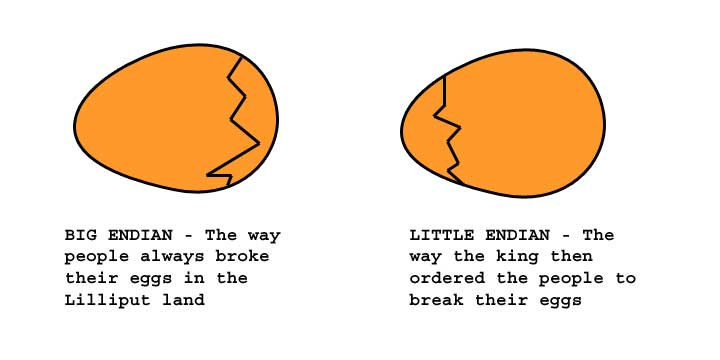
\includegraphics[scale=0.3]{eggs.jpg}
	\end{center}

	Есть два клана: little-endian (остроконечники) и big-endian (тупоконечники).
	По-русски всегда используют английские термины.
\end{frame}

\begin{frame}{Big-endian}
	Используется в низкоуровневых сетевых протоколах (TCP) и процессорах Atmel AVR (ATmega и прочие).

	Младший байт имеет больший адрес.
	Читается просто:
	\begin{center}
		\begin{tabular}{|c|c|c|c|l|}
			\hline
			\multicolumn{4}{|c|}{Адрес} & Значение \\
			& 2 & 3 & & \\\hline
			\dots & \t{0000 0001} & \t{0000 0011} & \dots & $\t{0000~00\textbf{01}~0000~00\textbf{11}}_2=259_{10}$ \\
			\hline
		\end{tabular}
	\end{center}

	Надо очень аккуратно помнить адрес и размер числа:
	\begin{center}
		\begin{tabular}{|c|c|c|l|}
			\hline
			\multicolumn{3}{|c|}{Адрес} & Значение \\
			& 2 & & \\\hline
			\dots & \t{0000 0001} & \dots & $\t{0000 0001}_2=1_{10}$ \\
			\hline
		\end{tabular}
	\end{center}
\end{frame}

\begin{frame}{Little-endian}
	Используется в x86: <<младший байт имеет меньший адрес>>.

	Читается хуже:
	\begin{center}
		\begin{tabular}{|c|c|c|c|l|}
			\hline
			\multicolumn{4}{|c|}{Адрес} & Значение \\
			& 2 & 3 & & \\\hline
			\dots & \t{0000 0001} & \t{0000 0011} & \dots & $\t{0000~00\textbf{11}~0000~00\textbf{01}}_2=769_{10}$ \\
			\hline
		\end{tabular}
	\end{center}
	Если только мы не Intel и не пишем к этому документацию:
	\begin{center}
		\begin{tabular}{|c|c|c|c|l|}
			\hline
			\multicolumn{4}{|c|}{Адрес} & Значение \\
			& \textbf{3} & \textbf{2} & & \\\hline
			\dots & \t{0000 0011} & \t{0000 0001} & \dots & $\t{0000~0011~0000~0001}_2=769_{10}$ \\
			\hline
		\end{tabular}
	\end{center}
	Они у себя всё пишут от старших к младшим: байты с меньшими адресами справа, младшие биты справа.
\end{frame}

\begin{frame}{Особенности Little-endian-1}
	Можно почти безболезненно конвертировать между типами:
	\begin{center}
		\begin{tabular}{|c|c|c|c|r|l|}
			\hline
			\multicolumn{4}{|c|}{Адрес} & \multicolumn{2}{|c|}{Значение} \\
			& 2 & 3 & & & \\\hline
			\dots & \t{0000 0011} & \t{0000 0001} & \dots & $\t{0000~0001~0000~0011}_2$ & $259_{10}$ \\
			\dots & \t{0000 0011} & \dots         & \dots & $\t{0000~0001}_2$           & $3_{10}$ \\
			\dots & \t{0000 0101} & \t{0000 0000} & \dots & $\t{0000~0000~0000~0101}_2$ & $5_{10}$ \\
			\dots & \t{0000 0101} & \dots         & \dots & $\t{0000~0101}_2$           & $5_{10}$ \\
			\dots & \t{1111 0011} & \t{0000 0000} & \dots & $\t{0000~0000~1111~0011}_2$ & $243_{10}$ \\
			\dots & \t{1111 0011} & \dots         & \dots & $\t{1111~0011}_2$           & $243_{10}$ \\
			\dots & \t{1111 0011} & \dots         & \dots & $\t{1111~0011}_2$           & $-13_{10}$ \\
			\dots & \t{1111 0011} & \t{1111 1111} & \dots & $\t{1111~1111~1111~0011}_2$ & $-13_{10}$ \\
			\hline
		\end{tabular}
	\end{center}
\end{frame}

\begin{frame}[t]{Особенности Little-endian-2}
	\begin{itemize}
		\item
			Есть проблема со знаком, если мы переходим от меньшего типа к большему.
		\item
			Надо \textit{расширять знак}, если у нас было знаковое число:
			заполнять старшие байты либо нулями, либо единицами (в зависимости от\only<1>{...}\only<2->{ старшего бита в числе}).
	\only<3->{
		\item
			Если число было беззнаковое, то надо старший байт заполнить нулями.
	}
	\end{itemize}

	\only<3->{
	Компиляторы низкоуровневых языков делают это автоматически, когда вы делаете какие-то присваивания.
	Разумеется, надо аккуратно следить за типами, иначе не сделают.

	Замечание: иногда, несмотря на тип \t{int}, какие-то функции могут ожидать в нём на самом деле не число,
	а набор байт в определённом порядке.
	Яркий пример "--- номер порта в работе с сетью на C, функция \t{htons} "--- это оно.
	}
\end{frame}

\begin{frame}{Резюме}
	\begin{enumerate}
		\item
			Целые числа хранятся в двоичной системе счисления.
		\item
			Знаковость числа определяется лишь типом данных.
		\item
			Самый распространённый способ кодирования отрицательных чисел "--- <<дополнительный код>>.
		\item
			В дополнительном коде старший бит отвечает за знак, а арифметика делатеся так же, как и в беззнаковых числах.
		\item
			Операциям сравнения чисел на меньше/больше и делению важно знать, работаем ли мы в дополнительном коде или с беззнаковыми числами.
		\item
			Порядок байт в числах может отличаться даже в разных местах внутри одного приложения.
			Читайте документацию, если работаете с чем-то на уровне байт!
		\item
			Если работаете с little-endian и меняете количество байт в числе "--- позаботьтесь о знаке.
		\item
			Если есть либо дополнительный код, либо переполнения, то важно количество бит/байт в числе.
	\end{enumerate}
\end{frame}

\section{Вещественные числа}
\subsection{Идеи}

\begin{frame}
	\tableofcontents[currentsection,currentsubsection]
\end{frame}

\begin{frame}
	Зачем нужны вещественные числа в компьютерах?
	Почему нельзя обойтись целыми?

	\pause
	\begin{itemize}
		\item Работа с дробями и деление.
		\item Денежные единицы: копейки удобно считать сотыми частями рубля.
		\item Физические (и военные) вычисления: тригонометрия, расстояния, геокоординаты.
	\end{itemize}
\end{frame}

\begin{frame}{С фиксированной запятой}
	\begin{itemize}
		\item
			Пример: рубли.
		\item
			После запятой всегда ровно два знака: $230.40$.
		\item
			По сути те же целые числа, только надо помнить, где стоит запятая, и перемножаются чуть по-другому (со сдвигом запятой и, соответственно, обрезанием знаков).
	\end{itemize}
	Есть в некоторых базах данных, используются как раз для хранения количества денег.

	Плюсы:
	\begin{itemize}
		\item Абсолютная точность, кроме, иногда, умножения и деления.
		\item Простые и предсказуемые операции.
		\item Простое описание допустимых значений.
	\end{itemize}
\end{frame}

\begin{frame}{Минусы}
	\begin{itemize}
		\item
			Надо заранее знать, сколько знаков потребуется.
		\item
			Если может требоваться разное число знаков в разных местах "--- надо брать разные типы данных и конвертировать.
		\item
			Соответственно, нужен разный код, если есть вычисления и с <<большими>> числами, и с <<маленькими>>.
		\item
			Не реализовать аппаратно, потому что неясно, сколько знаков отбрасывать при умножении;
			реализовывать много типов сложно.
	\end{itemize}
\end{frame}

\begin{frame}{С плавающей запятой}
	\begin{itemize}
		\item
			Обобщение числа с фиксированной запятой.
		\item
			Храним отдельно число и отдельно "--- сколько у нас знаков идёт после запятой, а сколько "--- до.
		\item
			Умножение и деление остались примерно такими же по сложности, а вот сложение и вычитание усложнились (надо сравнивать порядок чисел).
		\item
			Теперь можно делать вычисления с числами любого порядка, и будем знать порядок ответа и первые сколько-то цифр.
	\end{itemize}
	Плюсы:
	\begin{itemize}
		\item
			Одинаково хорошо работает и с маленькими, и с большими числами.
		\item
			Относительная погрешность вычислений сохраняется.
	\end{itemize}
\end{frame}

\subsection{Детали}
\begin{frame}{Первая попытка}
	Пусть храним числа так:
	\begin{gather*}
		x = a \cdot 10^{b} \\
		-32768 \le a, b \le 32767
	\end{gather*}
	Тут $a$ "--- \textit{мантисса}, $b$ "--- \textit{экспонента}.

	Например:
	\begin{align*}
		12.3 &= 123 \cdot 10^{-1} \\
		231000 &= 231 \cdot 10^3 \\
		12.3 \cdot 231000 &= 123 \cdot 10^{-1} \cdot 231 \cdot 10^3 = (123 \cdot 231) \cdot 10^{-1+3} = 28413 \cdot 10^2 \\
		12.3 + 231000 &= 123 \cdot 10^{-1} + 231 \cdot 10^3 = (123 + \underbrace{2310000}_{>>32767}) \cdot 10^{-1}
	\end{align*}
\end{frame}

\begin{frame}{Трудности с десятичной системой}
	\begin{itemize}
		\item При сложении у нас легко может произойти переполнение типа.
		\item Можно пытаться оставлять только самые значащие цифры.
		\item Но в общем случае надо домножать на большую степень десятки.
		\item Как это делать без очень больших чисел и без домножения на десятку каждый раз "--- неясно.
		\item Храним-то всё в двоичной системе, а там от умножения на десять меняется всё число.
	\end{itemize}
\end{frame}

\begin{frame}{Решение проблемы}
	Храним числа так:
	\begin{gather*}
		x = a \cdot \textbf{2}^b \\
		-32768 \le a, b \le 32767
	\end{gather*}
	\begin{itemize}
		\item Теперь стало легко и складывать, и перемножать, так как при домножении на двойку легко понять, сколько цифр не нужны.
		\item Можно реализовать в железе.
		\item
			Проблемы с тем, что нет чёткого соответствия между десятичными знаками после запятой и двоичными,
			нет точности:
	\end{itemize}
	\begin{align*}
		0.75_{10} &= {0.11}_{2} \\
		7 \cdot 10^{-1} + 5 \cdot 10^{-2} &= 2^{-1} + 2^{-2} \\
		0.1_{10} &= {0.000110011001100110011001101\dots}_{2} \\
		10^{-1} &= 2^{-4} + 2^{-5} + 2^{-7} + 2^{-8} + \dots \\
	\end{align*}
\end{frame}

\begin{frame}[fragile]{Упражнение}
	\begin{itemize}
		\item
			Введите в Python:
\begin{minted}{python}
x=0.1
print(x)
print(format(x, ".1000f"))
\end{minted}
		\item
			Убедитесь, что вы не получили \t{0.1}
		\item
			Найдите, на какую степень двойки надо домножить $x$, чтобы он стал целым.
			По сути "--- грубое приближение числа знаков в мантиссе.
	\end{itemize}
	\pause
	Ответ: на $2^{55}$.
	Из этого можно сделать вывод, что в мантиссе порядка $55$ знаков.
\end{frame}

\subsection{IEEE 754}
\begin{frame}
	\tableofcontents[currentsection,currentsubsection]
\end{frame}

\begin{frame}{Что такое IEEE 754}
	\begin{itemize}
		\item
			IEEE 754 "--- это стандарт хранения и обработки вещественных чисел с плавающей запятой, который используется почти везде.
		\item
			Но не вообще везде.
		\item
			Определяет несколько типов данных с разными размерами мантисс и экспонент: single precision, double precision, и ещё несколько.
		\item
			Достаточно разумно определяет операции для всех аргументов и решает некоторые проблемы.
		\item
			Из-за этого сложнее, чем идея с предыдущих слайдов.
		\item
			Есть $\pm \infty$, есть \t{NaN} (Not a Number, получается при делении нуля на ноль).
		\item
			В Python используется double-precision (тип \t{float}).
		\item
			В C++/Java есть как single-precision (\t{float}), так и double-precision (\t{double}).
	\end{itemize}
\end{frame}

\begin{frame}{Формат single-precision}
	Основная масса "--- \textit{нормализованные числа}:
	\begin{center}
		\begin{tabular}{c|c|c}
			\multicolumn{3}{c}{Биты} \\
			31 & 30-23 & 22-0 \\\hline
			знак ($s$) & экспонента ($e$) & мантисса ($m$) \\
		\end{tabular}
	\end{center}
	\begin{enumerate}
		\item
			Если $s=0$, то число положительное, иначе отрицательное.
		\item
			Предполагается, что экспонента подобрана так, чтобы перед запятой был ровно один знак "--- единица.
		\item
			Мантисса хранит все знаки \textit{строго после} этой единицы.
		\item
			Если $e=0$, то у нас число вида \t{1.1001010010} в двоичной записи (до запятой "--- ровно одна единица).
		\item
			Итоговая формула (для \textit{нормализованных} чисел):
			\[ x = (-1)^s \cdot 2^{e} \cdot (1 + m \cdot 2^{-23}) \]
	\end{enumerate}
\end{frame}

\begin{frame}{Хранение экспоненты}
	Экспонента хранится как беззнаковое число со сдвигом на 127:
	\begin{center}
		\begin{tabular}{r|l}
			Двоичное представление & $e$ \\\hline
			\t{0000 0000} & -127 \\
			\t{0000 0001} & -126 \\
			\vdots & \vdots \\
			\t{0111 1110} & -1 \\
			\t{0111 1111} & 0 \\
			\t{1000 0000} & 1 \\
			\vdots & \vdots \\
			\t{1111 1110} & 127 \\
			\t{1111 1111} & 128 \\
		\end{tabular}
	\end{center}
	Обратите внимание, что отрезок чисел "--- от $-127$ до 128, а не от $-128$ до $127$ (как в дополнительном коде).
\end{frame}

\begin{frame}{Пример}
	\[
		x = -13.75_{10} = \frac{-220}{16} = -1101.1100_2
	\]
	Подбираем экспоненту так, чтобы слева получилась ровно одна единица:
	\begin{align*}
		x &= -1.\underbrace{1011100_2}_{m'=184_{10}} \cdot 2^3 = \quad e=3 \\
		  &= -1.\underbrace{10111000000000000000000_2}_{m} \cdot 2^3
	\end{align*}
	Так как в $m$ предполагается 23 значащих знака (а у нас в $m'$ только 7), надо дописать \textit{справа} нулей.
	Итого:
	\begin{center}
		\begin{tabular}{c|c|c}
			\multicolumn{3}{c}{Биты} \\
			31 & 30-23 & 22-0 \\\hline
			\t{1} & $\underbrace{\t{100~0001~0}}_{e+127}$ & $\underbrace{\t{\textbf{101~110}0~0000~0000~0000~0000}}_{m}$ \\
		\end{tabular}
	\end{center}	
\end{frame}

\begin{frame}{Проблемы с аксиомами}
	Какое наименьшее нормализованное число можно представить в таком формате?
	Очевидно, при минимальной экспоненте (-127) и мантиссе.
	Тогда самые маленькие числа таковы:
	\begin{align*}
		x &= 2^{-127} \cdot 1 \\
		y &= 2^{-127} \cdot (1 + 1 \cdot 2^{-23}) \\
		z &= 2^{-127} \cdot (1 + 2 \cdot 2^{-23}) \\
		& \text{посчитаем что-нибудь:} \\
		y - x &= 2^{-127} \cdot (1 + 1 \cdot 2^{-23} - 1) = 2^{-127} \cdot 1 \cdot 2^{-23} = 2^{-150}
	\end{align*}
	Вопрос: как хранить $2^{-150}$?
	\begin{itemize}
		\item
			Округлять к $2^{-127}$ странно: это далеко; тогда бы получили, что $x-y=x$, но $x\neq x + y$.
		\item
			Округлять к нулю тоже странно: $x \neq y$, но $x - y = 0$.
	\end{itemize}
\end{frame}

\begin{frame}[fragile]{Денормализованные числа}
	\begin{itemize}
		\item 
			Вблизи нуля добавили \textit{денормализованные числа}, чтобы повысить точность и избежать подобных проблем с аксиомами.
		\item
			Теперь стандарт гарантирует, что $x - y = 0 \iff x = y$.
		\item
			Денормализованное число "--- это число с минимально возможной экспонентой, у которого отсутствует единица перед запятой:
			\begin{center}
				\begin{tabular}{r|r}
					Нормализованные   & $\t{\textbf{1}.\overbrace {0010011}^{m}} \cdot 2^{e=4}$ \\\hline
					Денормализованные & $\t{\textbf{0}.\underbrace{10010011}_{m}} \cdot 2^{e=5}$ \\
				\end{tabular}
			\end{center}
		\item
			Это просто $2^{23}$ чисел, равномерно распределённых от 0 до минимального нормализованного.
		\item
			Всё равно можно получить underflow:
\begin{minted}{python}
x=2**(-1074)
print(x, x / 2 * 2)
\end{minted}
	\end{itemize}
\end{frame}

\begin{frame}{Формат}
	Скажем, что если экспонента состоит из нулей, то у нас денормализованное число:
	\begin{center}
		\begin{tabular}{r|c|c|c}
			\multicolumn{3}{c}{Биты} \\
			31 & 30-23 & 22-0 \\\hline
			знак ($s$) & нули & мантисса $m$ \\
		\end{tabular}
	\end{center}
	Тут мы уже считаем, что мантисса записана целиком, включая старшую единицу.
	Формула:
	\[
		x = (-1)^s \cdot 2^{-12\textbf{6}} \cdot m \cdot 2^{-23}
	\]
	Тогда денормализованные числа лежат в диапазоне:
	\[
		2^{-126} \cdot 2^{-23} \le x \le 2^{-126} \cdot (2^{23}-1) \cdot2^{-23}
	\]
	А нормализованные "--- в таком:
	\[
		2^{-126} \cdot 1 \le x
	\]
\end{frame}

\begin{frame}
	\begin{center}
		
\includegraphics[scale=0.75]{what-are-you-doing.jpg}
	\end{center}
\end{frame}

\begin{frame}{Все особенности IEEE-754}
	Числа, доступные в IEEE 754 одинарной точности:
	\begin{center}
		\begin{tabular}{r|c|c|c}
			\multicolumn{3}{c}{Биты} & \\
			31 & 30-23 & 22-0 & Значение \\\hline
			\t{0} & \t{111 1111 1} & \t{000 0000 0000 0000 0000 0000} & $+\infty $\\
			\t{1} & \t{111 1111 1} & \t{000 0000 0000 0000 0000 0000} & $-\infty $\\
			\t{?} & \t{111 1111 1} & не нули                          & \t{NaN} \\
			\t{0} & \t{000 0000 0} & \t{000 0000 0000 0000 0000 0000} & $+0$ \\
			\t{1} & \t{000 0000 0} & \t{000 0000 0000 0000 0000 0000} & $-0$ \\
			\t{?} & \t{000 0000 0} & не нули                          & д. число \\
			\t{?} & что угодно     & что угодно                       & н. число \\
		\end{tabular}
	\end{center}	
\end{frame}

\begin{frame}{Упражнение}
	\begin{enumerate}
		\item
			Введите несколько простых десятичных дробей в Python и попробуйте методы \t{float.as\_integer\_ratio()} и \t{float.hex()}.
		\item
			Составьте таблицу сравнения для \t{0}, \t{+0}, \t{-0} на Python: кто кому равен, кто кого меньше.
		\item
			Добавьте в эту таблицу сравнения \t{NaN}.
		\item
			На C++/Python составьте таблицу уможнения для $\pm0$, $\pm 1$, $\pm \infty$ и \t{NaN}.
		\item
			На C++ составьте таблицу деления для этих же чисел (на Python некоторые операции вызывают исключение
	\end{enumerate}
\end{frame}

\subsection{Практические последствия}

\begin{frame}
	\tableofcontents[currentsection,currentsubsection]
\end{frame}

\begin{frame}[fragile]{Хранятся только старшие знаки}
\begin{minted}{python}
for a in [2.0 ** x for x in [10, 20, 40, 60, 1000]]:
    print(a == a + 1, a == a * (1 + 2 ** (-40)), a + 1 - a)
\end{minted}
	В Python у нас тип двойной точности, поэтому до $2^{40}$ единица ещё будет играть роль, а вот после "--- нет.

	Складывать/вычитать числа разных порядков "--- плохо.
	Сильно теряется точность.
\begin{minted}{python}
print(1000 + 1e100 - 1e100)
print(1e100 + 1000 - 1000)
\end{minted}
	Одного порядка "--- нормально.
\end{frame}

\begin{frame}[fragile]{Ошибка может копиться}
\begin{minted}{python}
from random import shuffle
a=[123456 * 2 ** x for x in range(0, 200)]
print(format(sum(a), ".20e"))  # Точный результат
a = list(map(float, a))
for _ in range(10):
    shuffle(a)
    print(format(sum(a), ".20e"))
\end{minted}
	\begin{itemize}
		\item
			Так как результаты округляются на каждом шаге, результат может зависеть от порядка вычислений, размеров чисел и фазы луны.
		\item
			Пример, где всё может быть плохо "--- метод Гаусса решения систем линейных уравнений (подробнее расскажут на алгоритмах).
		\item
			Уже для системы $15 \times 15$ можно подобрать матрицу, на которой точность теряется катастрофически быстро.
	\end{itemize}
\end{frame}

\begin{frame}{Оптимизатор}
	\begin{center}
		
\includegraphics[scale=0.4]{optimizer-game.jpg}
	\end{center}
\end{frame}

\begin{frame}{Оптимизатор}
	\begin{itemize}
		\item
			Часто процессор поддерживает числа большего размера, чем double-precision.
		\item
			Тогда точность может в некоторых местах случайно возрастать, а оптимизатор об этом не догадывается.
		\item
			Из-за этого <<побитово равные>> числа могут \href{http://codeforces.com/blog/entry/1059}{оказаться различными}:
			в одном месте сравнили куски памяти, а в других местах "--- лежащие в процессоре числа большей точности.
		\item
			Аналогично, можно случайно (не) увидеть какую-то маленькую погрешность.
	\end{itemize}
\end{frame}

\begin{frame}[fragile]{Десятичные дроби неточны}
\begin{minted}{python}
print(0.1 + 0.2)  # Классика
print(format(0.1 + 0.2, ".100f"))
print(format((0.1 + 0.2) * 2 ** 52, ".100f"))
for n in [1000, 1024]:
    fail, total = 0, 0
    for a in range(n):
        for b in range(n):
            if (a + b) / n != a / n + b / n:
                fail += 1
            total += 1
    print(fail, total, fail / total)
\end{minted}
\end{frame}

\begin{frame}{Что делать?}
	\begin{itemize}
		\item
			Не использовать вещественные числа.
		\item
			Особенно на контестах.
		\item
			Особенно у Серёжи.
		\item
			Если очень надо "--- готовиться к неточности и допускать погрешность при \textit{любых} сравнениях (см. оптимизатор):
			\begin{center}
				\begin{tabular}{c|c}
					Было & Стало \\\hline
					\t{a == b} & \t{abs(a - b) < eps} \\
					\t{a <= b} & \t{a <= b + eps}  \\
					\t{a < b} & \t{a < b - eps} \\
				\end{tabular}
			\end{center}
			Тут мы считаем, что числа равны, если отличаются не более, чем на \t{eps}.
		\item
			Следить за порядком операций и избегать сложения/вычитания чисел разного порядка.
		\item
			Иногда можно преобразовывать формулы: $x^2-y^2=(x-y)(x+y)$.
	\end{itemize}
\end{frame}

\begin{frame}{Замечания про сравнения}
	\begin{itemize}
		\item
			Можно сравнивать числа ещё аккуратнее, если смотреть на относительную погрешность, а не абсолютную.
			Или если надо сравнивать в программе и большие числа, и маленькие.
		\item
			Подбор \t{eps} и правильного порядка операций "--- отдельное искусство.
		\item
			Обычно на контестах берут \t{eps} от $10^{-5}$ до $10^{-15}$; мой любимый "--- $10^{-8}$.
		\item
			При желании может строго теоретически обосновать правильный \t{eps}.
		\item
			\pause
			Да и неправильный тоже :(
	\end{itemize}
\end{frame}

\begin{frame}[fragile]{Странные вычисления}
	Осторожно с \t{NaN}: любое вычисление с ним немедленно породит \t{NaN}, а сравнения с ним всегда выдают \t{false}:
\begin{minted}{python}
from math import sqrt
print(2 ** 1000 / 2 ** (-1000))
print(-2 ** 1000 / 2 ** (-1000))
print(sqrt(0), sqrt(2 ** (-1000)))
print(0 * float('inf'))
print(1 + float('nan'))
print(float('nan') == float('nan'))
\end{minted}
	В C++ его ещё можно получить, взяв корень из отрицательного числа или $\frac{0}{0}$ (Python может кинуть исключение).

	Лайфхак: когда извлекаете корень, не извлеките его случайно из \t{-eps}.
	Для этого стоит писать \t{sqrt(max(x, 0))}, если $x$ может быть близок к нулю.
\end{frame}

\subsection{Прочее безумие}

\begin{frame}
	\tableofcontents[currentsection,currentsubsection]
\end{frame}

\begin{frame}{Ручное округление}
	Самые популярные:
	\begin{center}
		\begin{tabular}{|c|c|c|c|c|}
			\hline
			\t{x} & \t{floor(x)} & \t{round(x)} & \t{ceil(x)} & \t{int(x) } \\\hline
			-1.6 & -2 & -2 & -1 & -1 \\
			-1.5 & -2 & -2 & -1 & -1 \\
			-1.4 & -2 & -1 & -1 & -1 \\
			-0.6 & -1 & -1 & 0 & 0 \\
			-0.5 & -1 & 0 & 0 & 0 \\
			-0.4 & -1 & 0 & 0 & 0 \\
			0.4 & 0 & 0 & 1 & 0 \\
			0.5 & 0 & 0 & 1 & 0 \\
			0.6 & 0 & 1 & 1 & 0 \\
			1.4 & 1 & 1 & 2 & 1 \\
			1.5 & 1 & 2 & 2 & 1 \\
			1.6 & 1 & 2 & 2 & 1 \\
			\hline
		\end{tabular}
	\end{center}
\end{frame}

\begin{frame}[fragile]{Последние замечания}
	\begin{itemize}
		\item
			Стандарт требует, что результат любой операции должен быть максимально точен, а округление должно быть до ближайшего числа.
		\item
			При этом округлять $\frac{1}{2}$ всегда вверх нехорошо "--- ошибка будет сильно накапливаться.
		\item
			Поэтому округляют до ближайшего чётного (<<банковское>> округление).
		\item
			Округление не знает про погрешность вычислений:
\begin{minted}{python}
from math import ceil
print(ceil(1))                  # 1
print(ceil(1.000000000000001))  # 2
\end{minted}
	Поэтому на практике, если могло получиться число, близкое к целому, лучше использовать \t{round} или добавлять \t{eps}.
		\item
			Не используйте типы с плавающей точкой для хранения количества денег или чего-то подобного, что требует точности при рассчётах.
	\end{itemize}
\end{frame}

\section{Дополнительные ссылки}

\begin{frame}
	\begin{enumerate}
		\item \href{http://acm.math.spbu.ru/~gassa/slides/number-representation.ru.pdf}{Презентация Ивана Казменко} (кружок при СПбГУ).
		\item \href{https://habrahabr.ru/post/112953/}{Статья на Хабре}.
		\item \href{http://www.softelectro.ru/ieee754.html}{Пересказ стандарта IEEE 754}.
		\item \href{https://www.h-schmidt.net/FloatConverter/IEEE754.html}{Онлайн-конвертер для single precision}.
		\item \href{http://steve.hollasch.net/cgindex/coding/ieeefloat.html}{Статья на английском}.
		\item \href{https://docs.python.org/3/tutorial/floatingpoint.html}{Документация Python на английском}.
	\end{enumerate}
\end{frame}


\end{document}
